\documentclass{article}

\usepackage{listings}
\usepackage{color}
\usepackage{graphicx}
\usepackage{titlesec}
\usepackage{amsmath}
\usepackage{hyperref}
\usepackage{amsmath}
\usepackage{graphicx}
\usepackage{subcaption}
\usepackage[title]{appendix}
\definecolor{dkgreen}{rgb}{0,0.6,0}
\definecolor{gray}{rgb}{0.5,0.5,0.5}
\definecolor{mauve}{rgb}{0.58,0,0.82}

\lstset{frame=tb,
  language=Python,
  aboveskip=3mm,
  belowskip=3mm,
  showstringspaces=false,
  columns=flexible,
  basicstyle={\small\ttfamily},
  numbers=none,
  numberstyle=\tiny\color{gray},
  keywordstyle=\color{blue},
  commentstyle=\color{dkgreen},
  stringstyle=\color{mauve},
  breaklines=true,
  breakatwhitespace=true,
  tabsize=3
}

\newcommand{\inlinecode}[2]{{\lstinline[language=#1]$#2$}}

\begin{document}

\title{%
  \textbf{Banknote Authentication Design Considerations} \\
  \large Machine Learning for Security and  \\
    Performance in Production Settings}
\author{Alice Chang, Karthik Umashankar, Yu Chen}
\maketitle

\begin{abstract}
Counterfeits have been an issue since the dawn of currency. While human analysts have historically been able to leverage the unique features of genuine banknotes to identify counterfeit, the prevalence of increasingly sophisticated scanning and printing technology has made the distinction far less discernable for the human analyst. This challenge was tackled previously by two researchers - Dr. Volker Lohweg and Eugen Gillich - who utilized a novel Shift-Invariant Wavelet Transform to obtain feature vectors representing the printed detail on both authentic and counterfeit banknotes; they were able to achieve 100\% classification accuracy using a Support Vector Machine with a second-order polynomial kernel\cite{original_paper}. The authors utilized an industry-standard technique of filtering the banknote grayscale image for viable regions of interest, and then performing a novel Shift Invariant Wavelet Transform for the model's feature engineering. We first validated Gillich and Lohweg's findings of 100\% accuracy on holdout datasets using a multitude of models (k-Nearest Neighbors, Support Vector Machine, etc.), and then identified critical thresholds where sample size begins to negatively impact the potential performance of a machine learning model once deployed into production.
\newline\newline
We conclude by investigating potential vulnerabilities an online machine learning system can encounter, specifically the Frog Boiling Attack. We outline a potential implementation of this type of penetration attack. In our experiments, depending on the classifier that was chosen, we were able to get the system to successfully mis-predict a forged data point as authentic in as few as 50 iterations. The complexity of the classifier did not offer better protection against the attack; simple models like k-Nearest Neighbors performed better than the Support Vector Machine \& Gaussian models.
\newline\newline
We also highlight various potential countermeasures to mitigate its negative impact on a machine learning system in production.
\end{abstract}

\section{Introduction}
According to US Federal Reserve, the \$20 is the most frequently counterfeited bill domestically. On the other hand, the \$100 note is the most frequently counterfeited bill internationally, with half to two-thirds of the \$900 billion value in circulation outside of the US\cite{intro_cite}. Recent technology has advanced to the point where the printing of high-fidelity counterfeit cash can be successfully achieved by a novice with a commonplace inkjet printer. Once counterfeit cash has been discovered in circulation, businesses and the general public bear the brunt of the resulting monetary loss, as the counterfeits are usually surrendered to law enforcement with no hope for reimbursement. Additionally, loss of currency credibility negatively impacts national creditworthiness, making accurate banknote validation a vital part of maintaining financial security.
\newline\newline
Many anti-fraud features have been added to currency, some of which include the 3-D security ribbon, color-shifting numbers, watermarking, and a UV-sensitive security thread. Interestingly enough, however, Dr. Lohweg and Mr. Gillich discovered that analyzing key features from a banknote's Intaglio printing technique is still fruitful even as the difference in quality between genuine and counterfeit currency becomes indistinguishable to the human eye.
\newline\newline
The Intaglio technique used within banknote printing allows for an unmatched sharpness in contrast through a feelable relief\cite{intaglio}. This technique forms a vital component of modern-day banknote authenticity verification. In the initial phase of authentication, \textbf{image digitization} occurs where the banknote relief is captured through industry-grade cameras to produce an image grayscale that can be then undergo a feature transformation, such as the Wavelet Transform (WT). Prior to feature transformation, various \textbf{Regions of Interest (ROI)}. Regions with low mean and variance in grayscale values of the various blocks are selected:
\begin{figure}
  \caption{A scatter plot from Gillich and Lohweg, 2010 showing the decision boundaries for selection of viable regions of interest. The circles are classified as appropriate ROIs while the squares are discarded for non-homogeneity or high mean grayscale values.}
  \centering
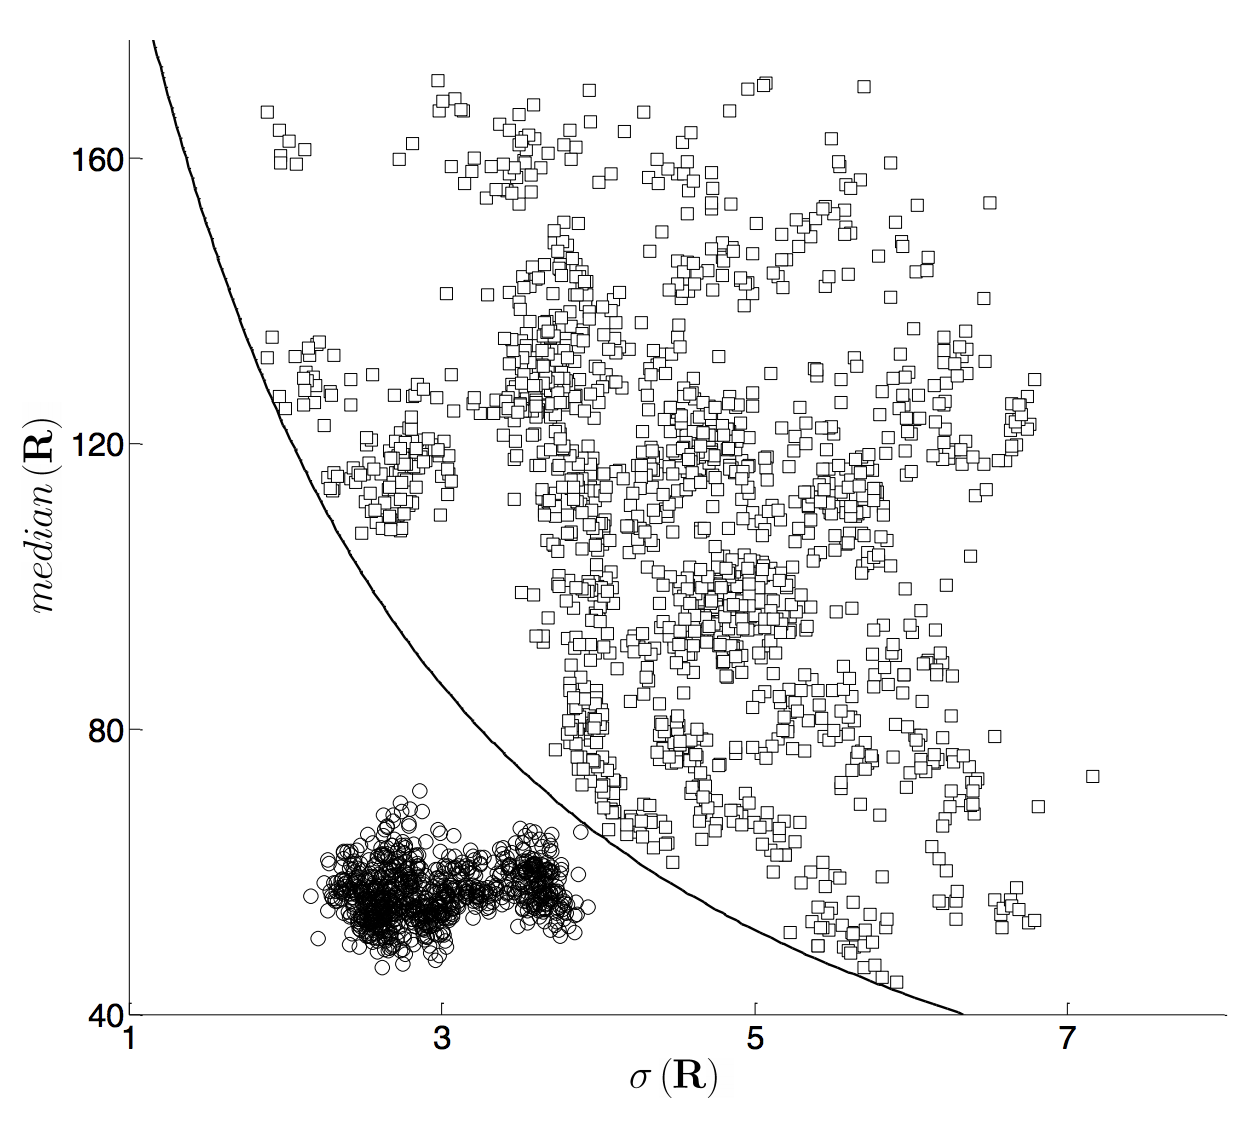
\includegraphics[width=80mm]{roi_selection.png}
\end{figure}
\newline\newline
We make use of their public data set to test out the performances of different classifiers, and take the resilient ones to task using the Frog Boiling Attack to measure their fragility. We also stress test the size of the data set to determine an optimal point between increasing the sampling size and the point of diminishing returns.
\section{Related Work}
As our work draws heavily on the previous research done by Dr. Lohweg and Gillich, it seems appropriate to explain their process in order to understand our data set. Their foundational premise is that the Intaglio printing technique, long used in the financial industry as a vital component to authenticity verification by providing unmatched sharpness in contrast and distinctive tactile qualities, could still be leveraged by machine learning to classify authentic banknotes from their counterfeit. Their work comprised of four parts: digitizing Regions of Interest (ROI) on a banknote, identifying the viable ROI from the unusable, dividing the regions into discrete sub-regions in grayscale, and using the median value and the standard deviations from the mean grayscale values as classifiable features. The ROI consisted of areas on the banknote where the printed image was detailed enough so as to capture a fairly uniform grayscale region with small standard deviation and low median value.
\begin{figure}
  \centering
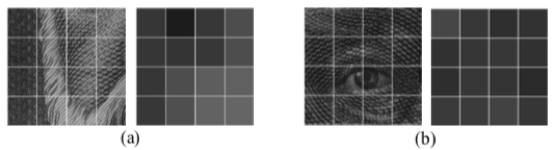
\includegraphics[width=80mm]{roi_distinguish.png}
  \caption{Distinguishing usefulness of ROI (left side) from their resulting mean values (right side): (a) is inhomogeneous and contains a more varied printing structure; (b) has a fairly uniform mean grayscale value and is ideal for authentication.}
\end{figure}
\newline\newline
When charted, the viable and unusable regions were unambiguous (See Fig. 1). The researchers then applied their novel two-dimensional wavelet transform (the Shift Invariant Wavelet Transform) to capture the scaling and structure of these ROIs and analyze the resulting statistical features from the standardized histograms of the wavelet coefficients 
\begin{figure}
  \centering
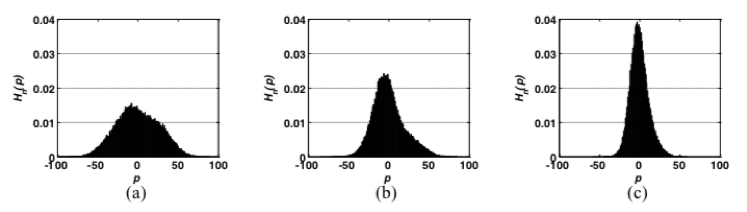
\includegraphics[width=80mm]{histogram.png}
  \caption{Histogram of wavelet coefficients after SWT: (a) from Genuine banknote; 
(b) from High-Quality forgery; and (c) from Low-Quality forgery.}
\end{figure}
\newline\newline
Additionally, using the Support Vector Machine polynomial kernel model to find clusters provided very clear classification between forged and genuine banknotes, with two discarded outliers that were ignored due to ambiguity of their appropriate classification.
\begin{figure}
  \centering
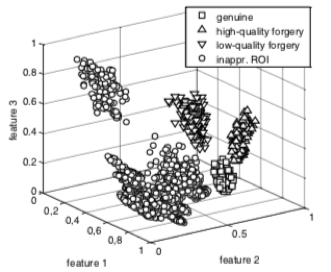
\includegraphics[width=80mm]{feature_space.png}
  \caption{Feature space using variance (feature 1), skewness (feature 2), and kurtosis (feature 3)}
\end{figure}
\newline\newline
The resulting 1371 data points' extracted features became the starting point of our research. 

\section{Experiments}

\subsection{Validation of Model Performances}
In their original paper, Gillich and Lohweg assert that 100\% accuracy can be achieved as a result of judicious Region of Interest selection and the Shift Invariant Transform. To validate, we performed basic data processing, scaling the dataset so that each feature column $k$ had $\mu_{k} = 0$ and a $\sigma_{k} = 1$:
\newline\newline
\begin{lstlisting}
import pandas as pd
import numpy as np
from sklearn.model_selection import train_test_split
from sklearn.preprocessing import StandardScaler

df = pd.read_csv("data/dataset.csv", encoding="latin-1") # import the CSV dataset and save as a Pandas dataframe object
    
targets = df["class"].values # save the targets (Y) as a NumPy array of integers
features_df = df.loc[:, df.columns != "class"] # save everything else as the features (X)
    
features_names = features_df.columns.values # save the column names
features_matrix = features_df.values # convert X from a dataframe to a matrix (for our machine learning models)
scaled_features_matrix = StandardScaler().fit_transform(features_matrix) # scale the data so mean = 0, unit variance - important for many models
\end{lstlisting}
The cleaned \lstinline{scaled_features_matrix} Numpy object can then be fed into a variety of different models:
\begin{lstlisting}
logistic_regression = LogisticRegression()
logistic_regression.fit(X_train, y_train)
training_predictions = logistic_regression.predict(X_train)
test_predictions = logistic_regression.predict(X_test)

# check accuracy of Logistic Regression
number_correct = np.sum(training_predictions == y_train)
number_correct_test = np.sum(test_predictions == y_test)
\end{lstlisting}
The fact that we were able to achieve 100\% accuracy on holdout sets speaks to the effectiveness of the feature engineering mechanism that Gillich and Lohweg utilized. Their Region of Interest selection methodology, combined with Shift Invariant Transform, takes a highly dimensional data (grayscales of banknote images), and partitions the data so clearly based upon the decision boundary of authenticated/forged that even basic linear classifiers such as the Logistic Regression are able to achieve remarkably strong classification performance.

\subsection{Sample Size Stress Testing}
\subsubsection{Overview}

Deployment of any machine learning authentication model requires strict thresholds for accuracy and overall performance. In the case of sensitive data protection and validation like banknote authentication, data scientists wish to minimize not only misclassifications, but false positives. A false positive results in a significant amount of financial loss, and potential damage to an institutions brand or public image if security loopholes are made public.

\subsection{Experimental Procedure}

We ran multiple iterations of our models (K-Nearest Neighbors, Gaussian Mixture Model, Support Vector Machine, Neural Network) across multiple different segmentations of train/test splits. We then measured the accuracy at each iteration and visualized the degradation of performance on both the test and training datasets.

\subsection{Experimental Results}

We found that elbow points in drops of accuracy existed for most classifiers as we increased the percentage of the data points allocated towards the test set. The green triangles below show performance on the training set, and the red circles show performance on the test set.
\begin{figure}
\centering
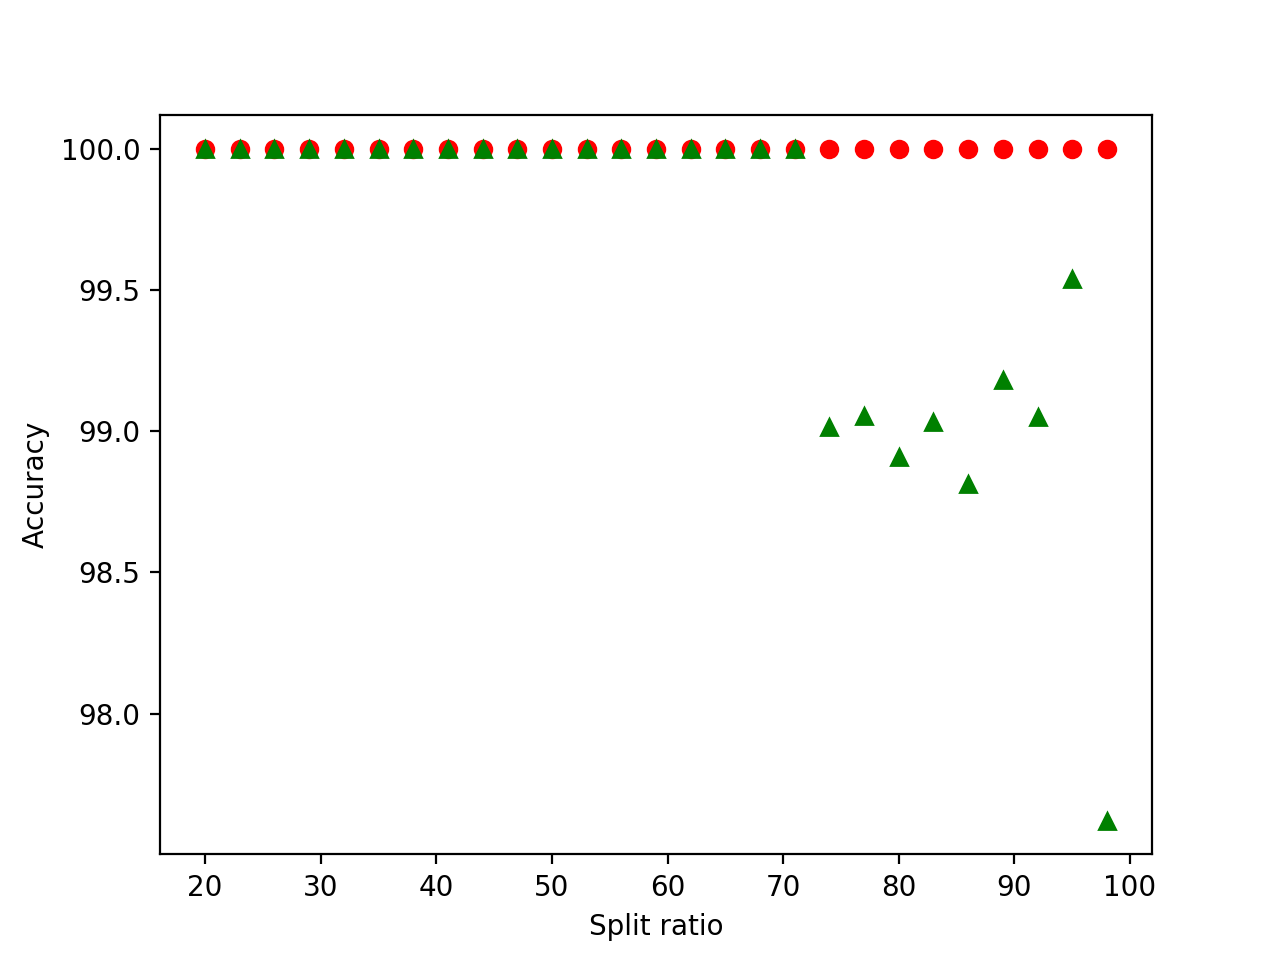
\includegraphics[width=60mm]{NN.png}
  \caption{Neural Network performance as training samples decrease.}
  \end{figure}
  \newline
\begin{figure} 
\centering
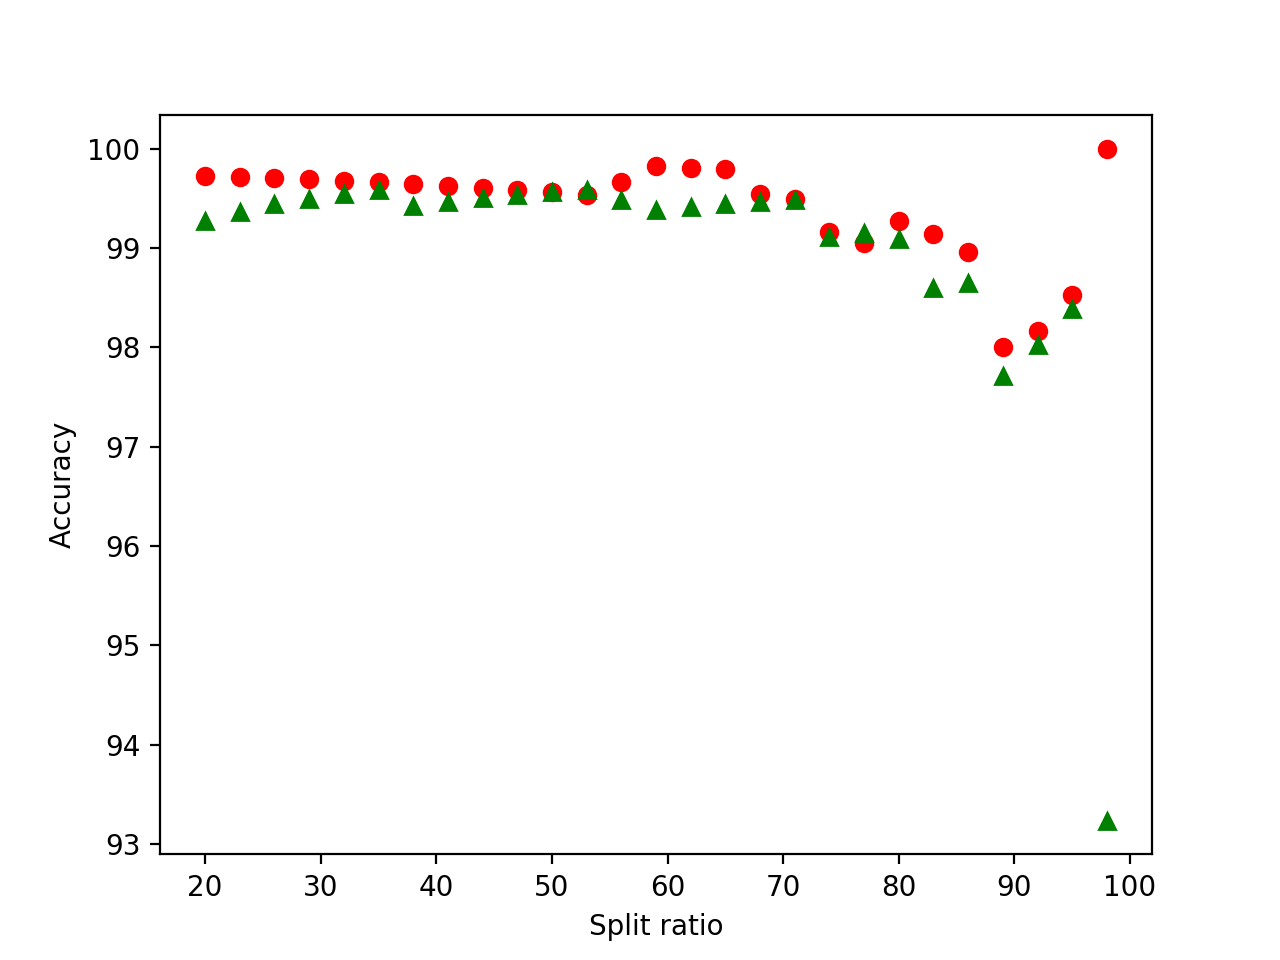
\includegraphics[width=60mm]{gaussian.png}
  \caption{GMM performance as training samples decrease.}
    \end{figure}
      \newline
    \begin{figure}
    \centering
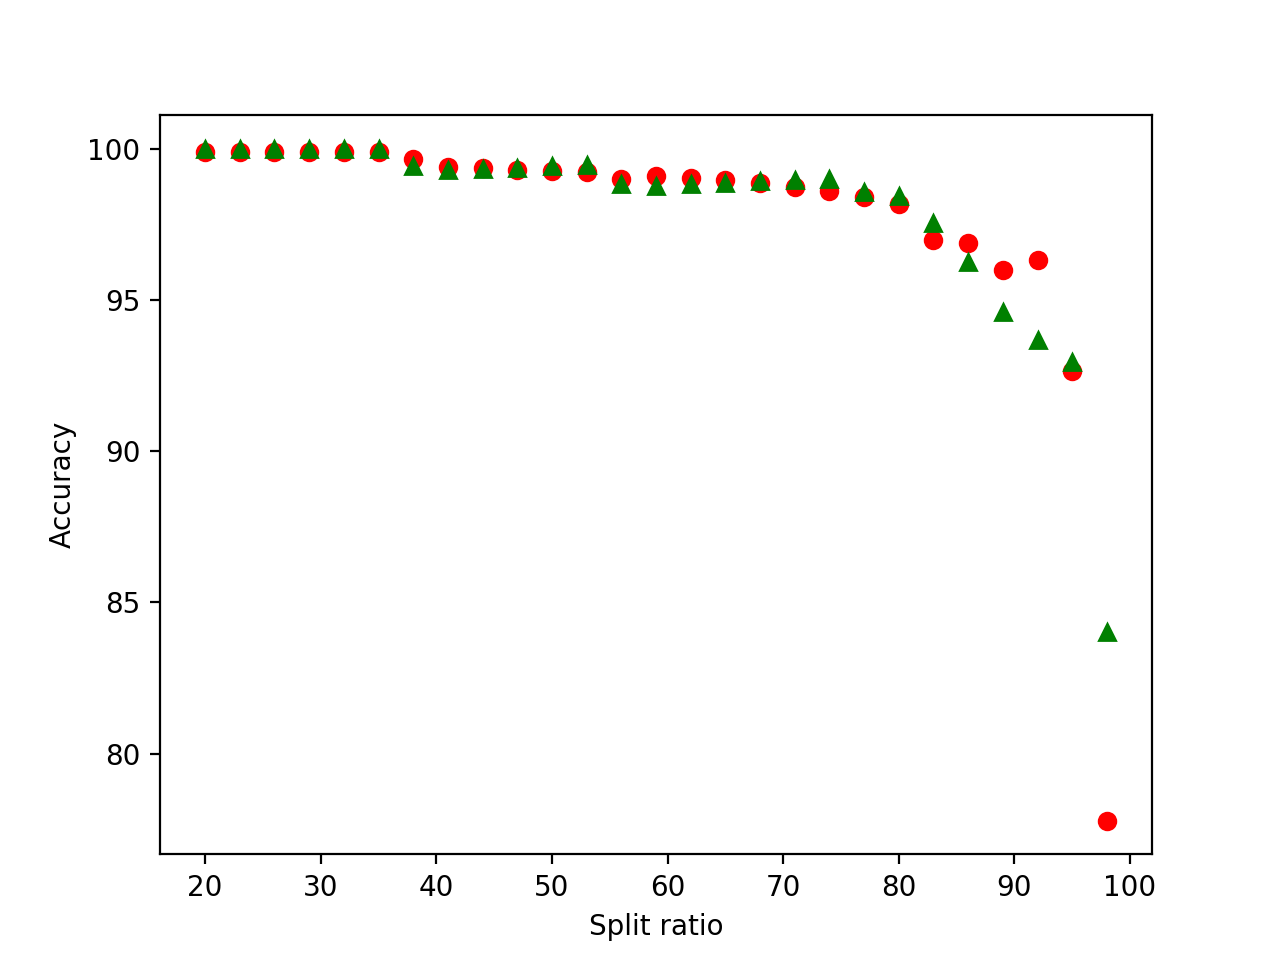
\includegraphics[width=60mm]{KNN.png}
  \caption{KNN performance as training samples decrease.}
      \end{figure}
        \newline
          \begin{figure}
          \centering
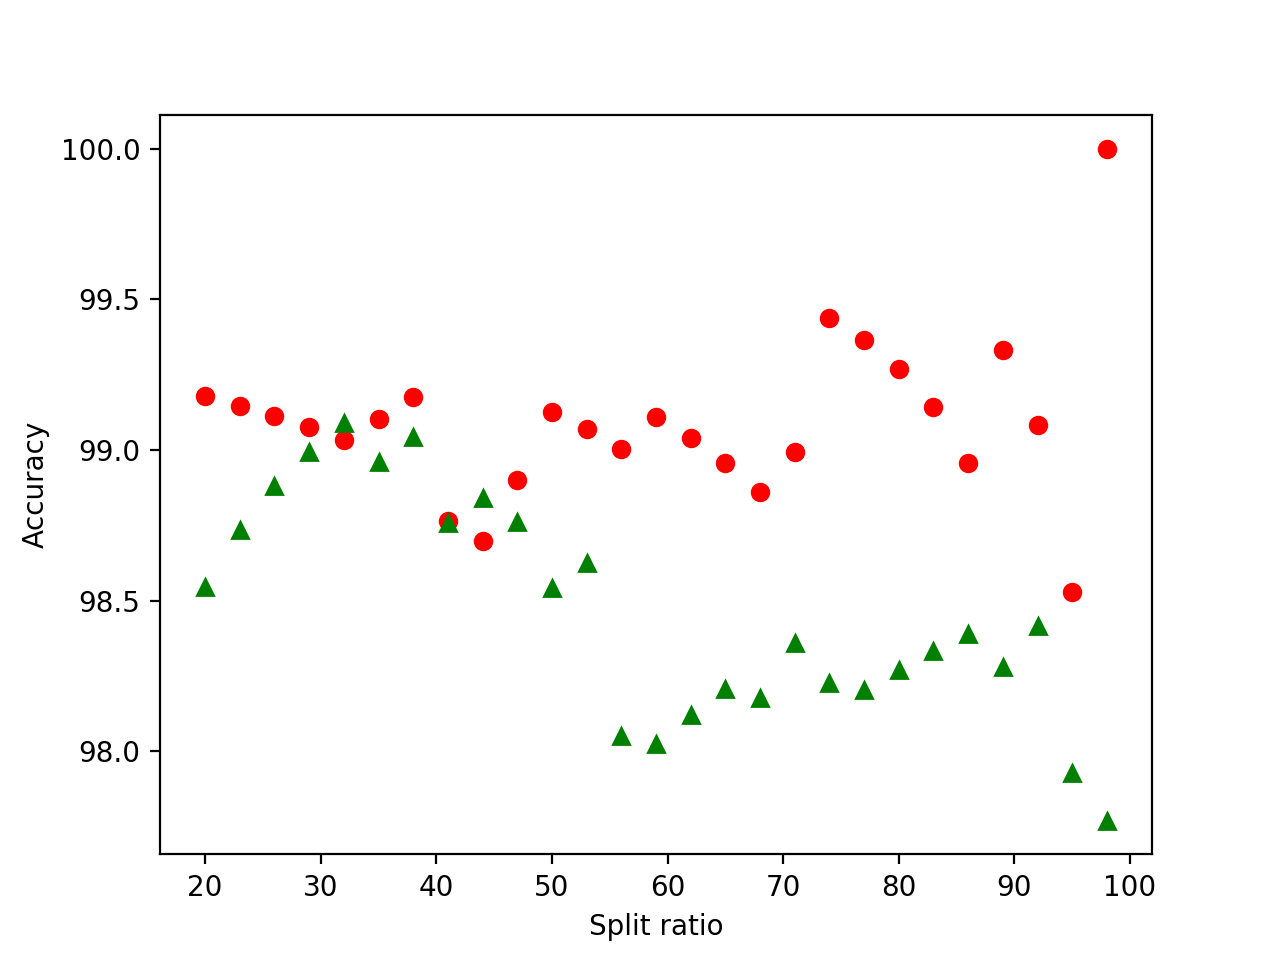
\includegraphics[width=60mm]{linear.png}
  \caption{SVC performance as training samples decrease.}
        \end{figure}
\newline\newline
Our results suggest that more robust and complex models, such as the neural network, are able to generalize the decision boundaries between authenticated and forged banknotes even with relatively few data samples. In our example, we typically saw accuracy begin to drop significantly when 70\%-80\% of the dataset was allocated towards testing (especially for the K Nearest Neighbors and Gaussian Mixture Model). Given our initial dataset size of 1,500 points, this suggests that there is a significant dropoff in performance with training samples under 500 points.

\subsection{Implementation of Frog Boiling Attack (FBA)}
\subsubsection{Overview}
The Frog Boiling Attack is most effective during business contexts where online learning occurs (when data arrives as a stream and becomes ingested sequentially, with the fitted model updated after each new data point). The attack relies upon the concept of template drift\cite{template_drift}, where the model's fitted "template" of an authentic banknote data sample is corrupted over time by a stream of compromised data points. The overall implementation, implemented over $N$ steps, relies upon the update equation

\begin{equation}
F_{new} = F_{old} + (i - 1)\delta(x)
\end{equation}

where

\begin{equation}
\delta(x) = \frac{\bar{x}_{target}-\bar{x}_{original}}{N}
\end{equation}

\subsubsection{Experimental Procedure}

In our experiments, we determined that the value of $\delta(x)$ is quite crucial in mounting a successful frog boiling attack. The idea behind the attack is to pass off forged banknotes as authentic, so, we should try to get the classifier to determine as many forged notes in the test data set as possible, as authentic. For this reason, for the remainder of this paper, when we refer to the authentic data set ($A_{data}$), it refers to the records in the training set that were classified as authentic, and when we refer to the forged data set ($F_{data}$), it refers to the records in the test set that were classified as forged.
\newline\newline
In each iteration, we start off by calculating the mean (centroid) of all values in $F_{data}$, and find the point in $A_{data}$ that's closest to the centroid, let's call it CAD (closest authentic data point). We then generate a new fake data point (FDP) by adding a tiny incremental value to the CAD. This incremental value is given by the formula

\begin{equation}
\frac{D_{CAD,F-CEN}}{N}
\end{equation}

where $D_{CAD,F-CEN}$ is defined as the Euclidean distance between the closest authenticated data point and the center of the trained forged data.
\newline\newline
We then add this new FDP back into $A_{data}$, manually assign it a classification of authentic, refit the model, and predict the classification of the FDP. If the classification is forged, we stop right there (as our attack is compromised). If the classification is authentic, we proceed to the next iteration.
\newline\newline
With the above-mentioned approach, we were able to successfully "attack" the system into incorrectly predicting a forged banknote as authentic. We ran the algorithm against five different classifiers, and some of them displayed a stronger aversion to false detection than the others, but with enough iterations, we were able to crack them all eventually (with the exception of the Random Forest classifier). The tables below detail the results, with the highlighted row indicating where we saw a drop in the accuracy.

\subsubsection{FBA Experimental Results}
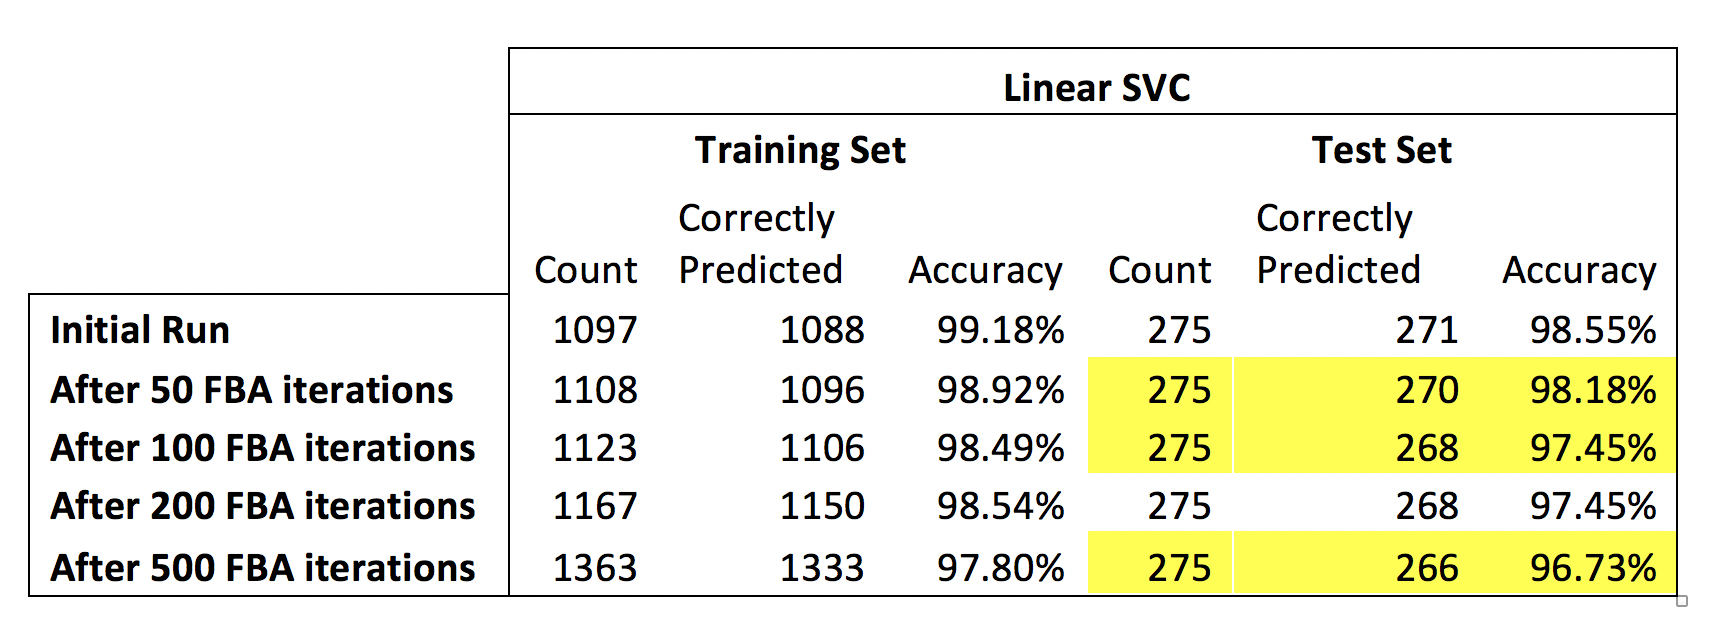
\includegraphics[width=125mm]{linear_svc_results.png}
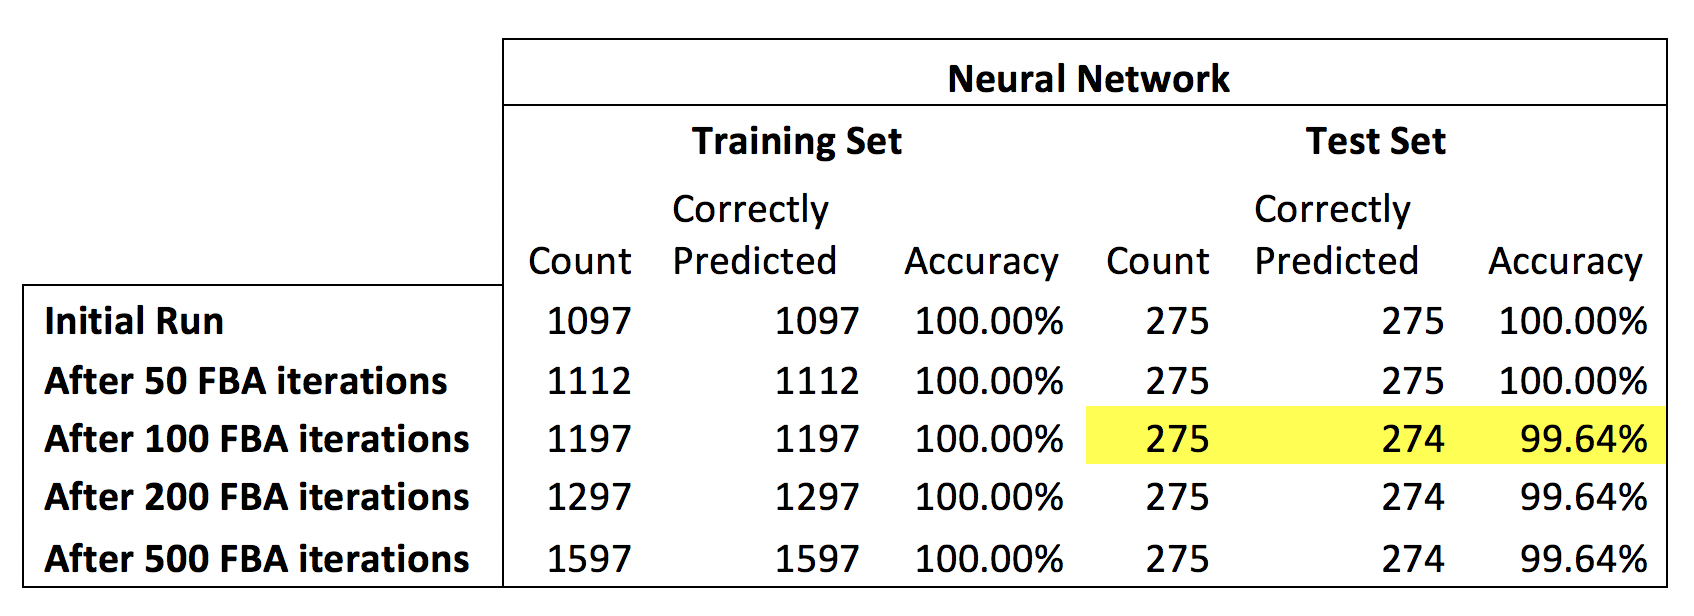
\includegraphics[width=125mm]{neural_network.png}
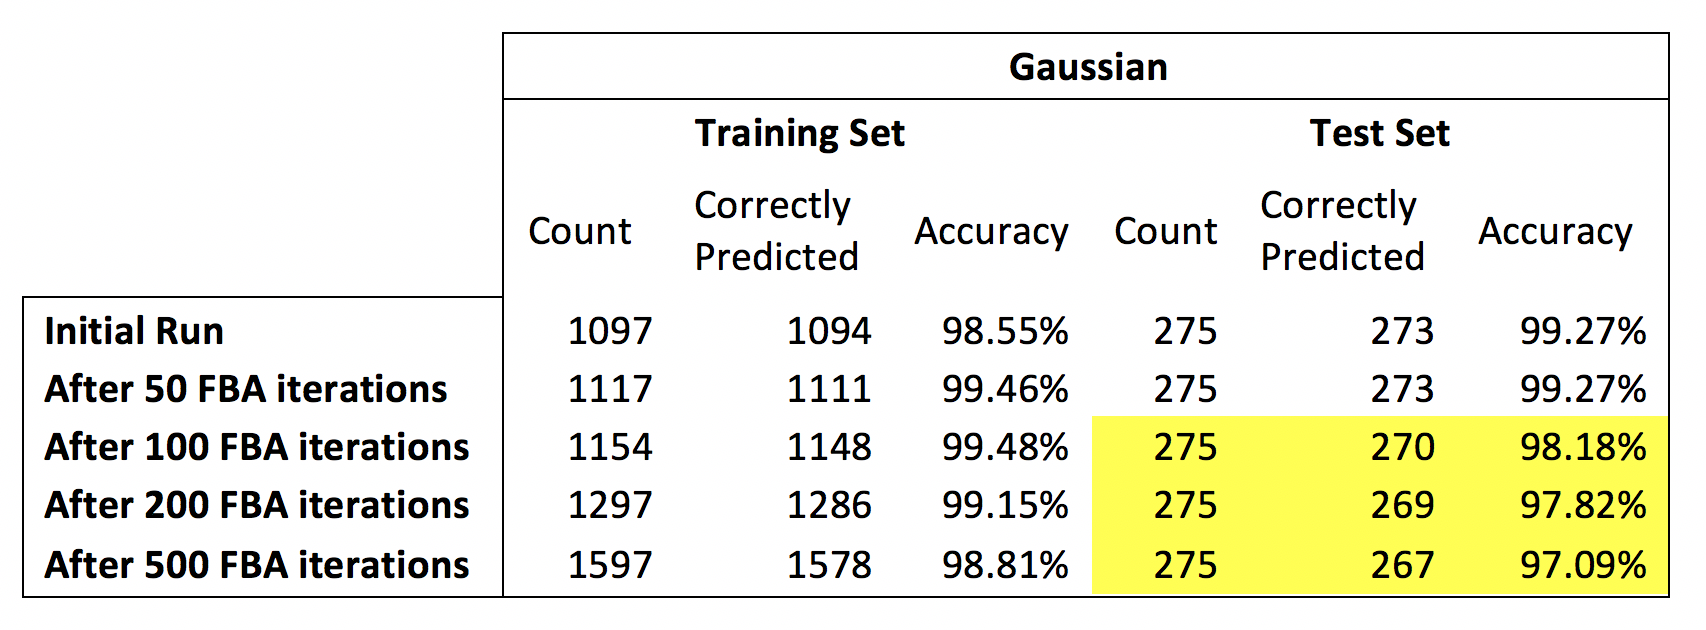
\includegraphics[width=125mm]{gaussian_results.png}
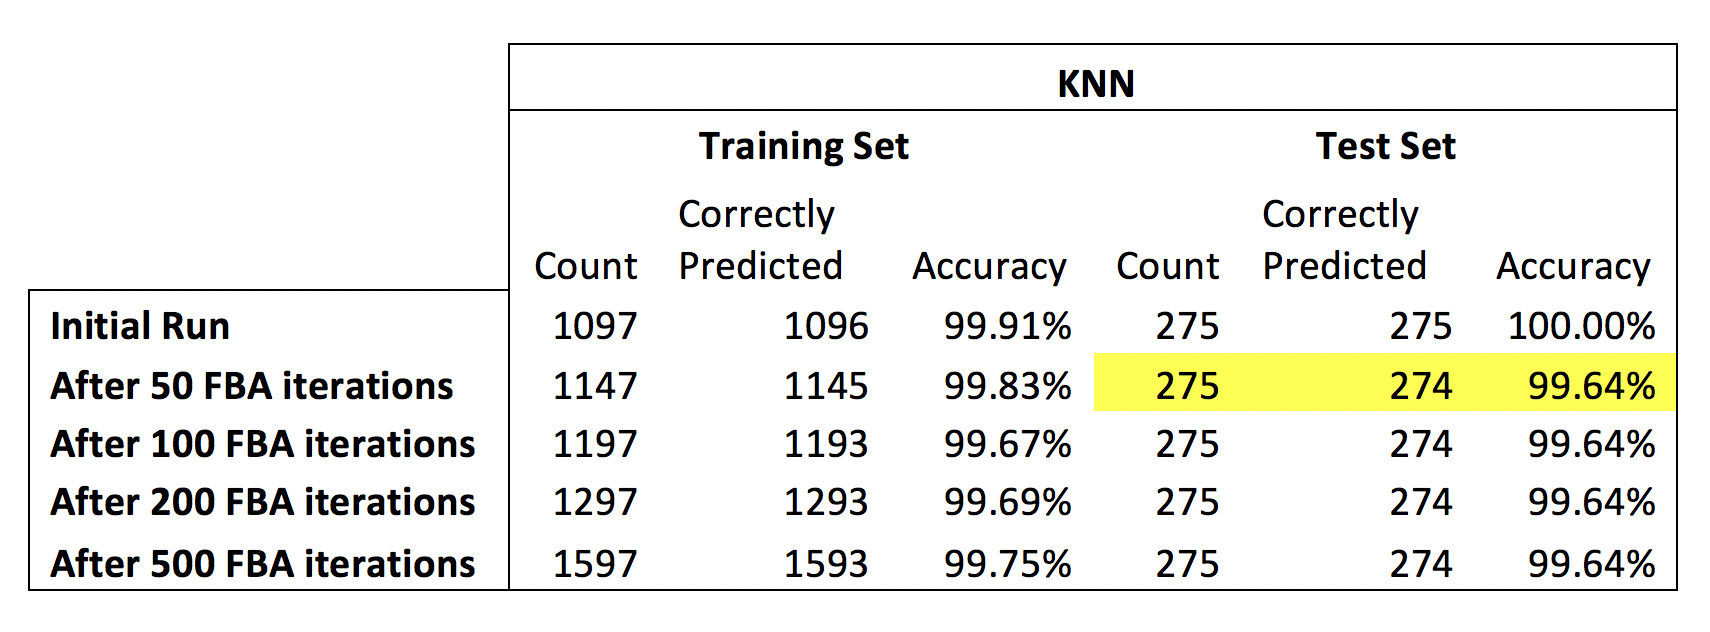
\includegraphics[width=125mm]{knn_results.png}
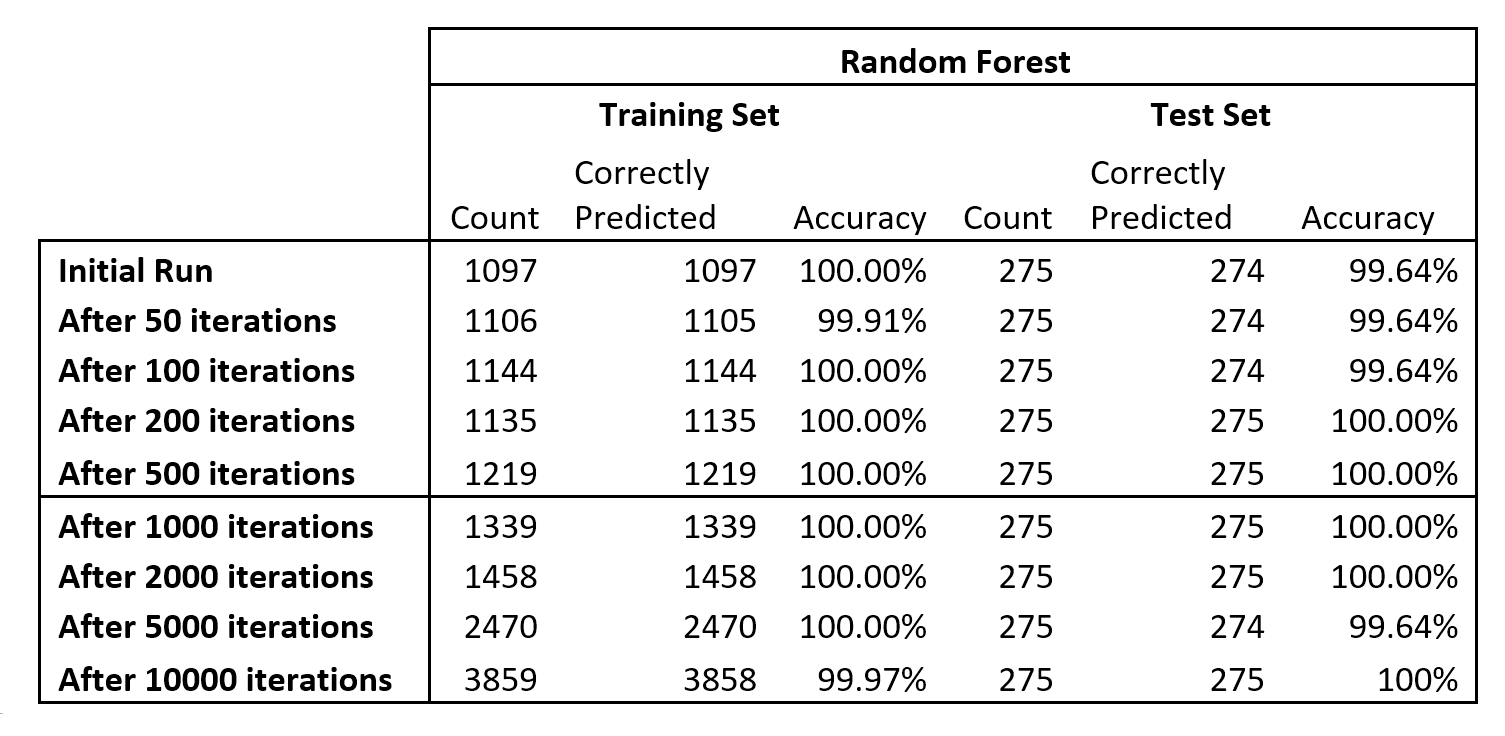
\includegraphics[width=125mm]{rf_results.png}

\subsubsection{Analysis of FBA Experimental Results}

\begin{itemize}
\item With the Neural Network and the KNN classifiers, since we drifted $A_{data}$ towards the mean of $F_{data}$, post the attack, it was only the data point closest to the mean that was classified as authentic. For the attack to succeed on several data points, we need to run it multiple times, once each towards the forged datapoint we want the system to misclassify.
\item With the Gaussian and the LinearSVC classifiers, with increasing iterations, we were able to classify more of $F_{data}$ as authentic. 
\item The LinearSVC model chosen by the original researchers performed the worst, with as many as 9 mispredictions post 500 iterations of the attack.
\item The Random Forest classifier really surprised us by almost always thwarting the attack at around the 30\% mark of the number of iterations. The initial count for the number of data points in the $A_{data}$ is \textit{1097}. For classifiers like KNN (that never detected the "corrupt" data points we were introducing as forged) you can see that at the end of n iterations, the number of data points in the $A_{data}$ set had increased to \textit{1097 + n}. Whereas in the case of Random Forest, even setting the iteration count to as high as 10000 only resulted in the classifier detected the corrupt data point after \~2700 iterations. Not only that, but its test and training accuracy seemed to get better the more iterations we ran.
\item We were able to reproduce the attack by starting with the mean value of $A_{data}$, rather than choosing the point closest to $F_{data}$, but it required significantly higher number of iterations (20x) to achieve the same result.
\end{itemize}

\subsubsection{FBA Countermeasures}

\begin{itemize}
  \item \textbf{Freezing Online Learning}: When discussing potential countermeasures to FBA, a tradeoff between responsiveness and security must be established. An obvious, yet sometimes unrealistic, method of prevention is to fully disable online learning completely, and "freeze" the authentication classifier. In many businesses cases, disabling online learning may result in a significant decline in model performance, especially if the feature space is exceptionally dynamic (ie. consumer entertainment and purchasing behavior, which is often a function of seasonality and inherent "drift").
  \item \textbf{Autocorrelation Detection}: An "honest" user (one who is utilizing the business' services as intended) should display no correlation between her submitted banknote data points. No correlation between a user's data points over time equates to each banknote being submitted independently of the prior banknotes (which should be the case if no fraudulent activity is happening).
  \newline\newline
  Autocorrelation functions are commonly used within time-series analysis to identify specific ranges of time periods that are indicative of future trends or behavior. ACF is also used as a metric for approximating the convergence of a Markov Process, specifically a Markov Chain Monte Carlo's stationary distribution\cite{mcmc}.
  
  \begin{figure}
  \centering
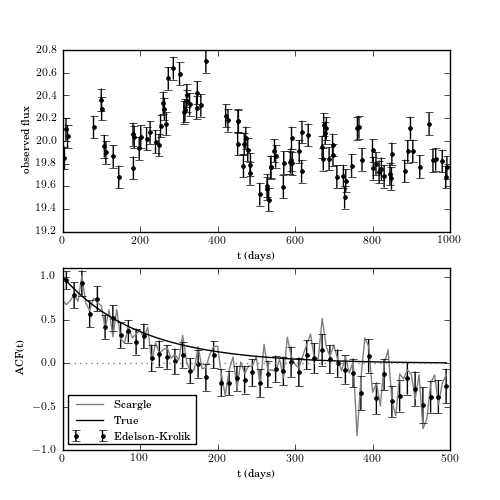
\includegraphics[width=80mm]{acf.png}
  \caption{An example of a typical autocorrelation function plot used to detect stationarity across time series data.}
\end{figure}

A crude, baseline implementation can be adopted to identify users perpetuating fraudulent banknotes:
\begin{itemize}
\item For each user, plot autocorrelation function across a reasonable time interval. There should be no autocorrelation, or the autocorrelation should decay rapidly.
\item For users flagged as having abnormal autocorrelations, identify how closely correlated the direction of movement is with the distance vector (a vector of differences between the negative centroid and the closest authenticated points).
\item If the traversal vector and the user's drifted banknote data points are highly correlated, this person is a prime candidate for submitting forged banknotes and further investigation is required.
\end{itemize}
  
\item \textbf{Batch Model Updates}: The crux of the Frog Boiling Attack is the assumption that the model will not be able to detect small "drift" towards a target template, capitalizing upon the inherent responsiveness of the model towards new data points. However, batching model updates increases the magnitude of "drift", with the hope being that the model is able to successfully detect larger "steps" if we perform model updates in batches. The pseudocode implementation for batching would be as follows:
\begin{lstlisting}
for user in users:
	BATCH_SIZE = 30 # update after user has submitted 30 banknotes
	batched_datapoints = [] # create a cache of datapoints per user
	authenticated = receive_data(banknote_datapoint) # ingest datapoint when user submits banknote
	
	if banknote_datapoint is authenticated:
		batched_datapoints.append(banknote_datapoint)
	else:
		batched_datapoints = [] # if any authentication points fail, clear the cache
		
	if length(batched_datapoints) == BATCH_SIZE: # once cache hits batch size, update the global model
		update_model(batched_datapoints)
\end{lstlisting}
Within this particular implementation, a key hyperparameter to optimize is \lstinline!BATCH_SIZE! This is the number of drift steps taken from the original template to the target template \textit{without updates (ie. model refitting)} before the model returns a negative classification. For instance, in our implementation of frog boiling attack, disabling the online learning model refitting and thereby freezing the model, we receive the following log output:
\begin{verbatim}
Closest positive point: [ 0.13 0.01 -0.54 0.24]
Negative centroid: [ 0.65 0.40 -0.14 0.02]
Distance from negative centroid: 0.79
Prediction: [0]
Classified as negative during iteration 10
\end{verbatim}
The simple k-Nearest Neighbors model will accept drift up to 10 steps away before it detects a fraudulent banknote datapoints. Thus, we'd likely set our \lstinline!BATCH_SIZE! to a number significantly higher than 10. This number can be set by repeatedly probing the authentication model with online learning disabled to generate a distribution of \textbf{tolerance thresholds}, or the number of steps taken before the machine learning begins to classify data points as negative. Say we have taken 50 different probes of our model, and the following array of tolerance thresholds are returned:

\begin{verbatim}
[ 7., 4., 2., 9., 13., 9., 10., 9., 13., 8., 8., 14., 8.,
10., 3., 12., 9., 15., 12., 8., 8., 13., 10., 5., 8., 15.,
6., 14., 8., 8., 15., 6., 6., 6., 15., 5., 11., 10., 9.,
13., 10., 13., 7., 9., 8., 11., 15., 8., 10., 16.]
\end{verbatim}

We can fit these results to a Gaussian distribution, and then find its inverse cumulative distribution function (ICDF) at an acceptable $\alpha$ level. In the context of banknote authentication, given the sensitive nature of financial assets at risk, a relatively stringent $\alpha$ can be selected of 0.001:
\begin{lstlisting}
from scipy.stats import norm
alpha = 0.001
fitted_mean = 10
fitted_standard_deviation=3
threshold = int(norm.ppf(1-alpha, loc=fitted_mean, scale=fitted_standard_deviation))
print(f"Batch size at alpha level {alpha} is {threshold}")
# Batch size at alpha level 0.001 is 17
\end{lstlisting}

Thus, a \lstinline!BATCH_SIZE! of 17 is selected for production deployment to minimize the risk of online learning intrusion attacks like FBA.

 \end{itemize}


\section{Future Work}
There is a healthy amount of research going into detecting counterfeit currency with machine learning, much of which leverage some variation of printing noise (such as our research), but there is also UV reactivity feature detection, as well as electromagnetic conductivity on various regions of a bill. It would be interesting to see whether the inclusion of these features would further strengthen or degrade the results of a classifier.

Furthermore, as a lot of these features require use of some sophisticated or commercial-grade equipment to extract the needed level of detail, more research could be done into the feature extraction and resulting accuracy rates of methods more available to the general populace - such as feature extraction using a camera in a mobile device. After all, small businesses and individuals also have a vested interest in ensuring the authenticity of the currency passing through their hands.
\begin{appendices}
\section{Python Source Code}
\subsection{Sample Size Stress Testing}

\begin{lstlisting}
if __name__ == "__main__":
    cl = BanknoteClassifier(dataset='data/dataset.csv')
    plotthis = []
    # for each classifier of our choosing
    for cname in ['knn', 'linear', 'random_forest', 'neural_network', 'gaussian']:
        # interate 100 times, classifying, and corrupting the dataset using previous classification results
        split = []
        train_accuracy = []
        test_accuracy = []
        print("Classifier: {}".format(cname.upper()))
        i=0
        for trainset in range(20, 100, 3):
            i += 1
            cl.adjust_train_test_split(trainset*0.01)
            result = cl.Classify(classifier=cname)
            # ---- iterative debugging ----
            # print("--- Iteration {} ---".format(i))
            # print_data('Training', result['training'])
            # print_data('Test', result['test'])
            # ---- json printout ----
            run = {
                'classifier': cname,
                'train/test split': '{}%'.format(trainset),
                'train set': result['training']['total_count'],
                'train accuracy' : result['training']['accuracy']*100,
                'test set' : result['test']['total_count'],
                'test accuracy' : result['test']['accuracy']*100
            }

            # ---- X/Y plotting ----
            split.append(trainset)
            train_accuracy.append(run['train accuracy'])
            test_accuracy.append(run['test accuracy'])
            print(json.dumps(run, indent=3))

        plot.plot(split, train_accuracy, 'ro', split, test_accuracy, 'g^')
        plot.xlabel('Split ratio')
        plot.ylabel('Accuracy')
        plot.show()
\end{lstlisting}

\subsection{Implementation of Frog Boiling Attack}
\begin{lstlisting}

    def CorruptData(self):
    
        """
        Finds the closest authenticated datapoint (CAD), negative centroid, and the traversal distance vector
        """

        negative_means = self.GetMean('training', 0)
        positive_means = self.GetMean('training', 1)

        training_df = pandas.DataFrame(self.training_features)
        training_positives_df = training_df[self.training_class == 1]

        current_distance = 9999
        closest_positive = None
        for i in range(training_positives_df.shape[0]):
            data_point = training_positives_df.values[i,:]
            distance = numpy.linalg.norm(data_point - negative_means)
            if distance < current_distance:
                closest_positive = data_point
                current_distance = distance

        print(f"Closest positive data point is {closest_positive}")

        distance = closest_positive - negative_means
        return closest_positive, distance, negative_means
        
    def GetMean(self, dataset, classification):

        """
        :param dataset: string option of either test or training
        :param classification: integer 0 or 1 to denote negative or positive
        """
        if dataset == 'test':
            class_source = self.test_class
            feature_source = self.test_features

        elif dataset == 'training':
            class_source = self.training_class
            feature_source = self.training_features
        targets = class_source == classification
        df = pandas.DataFrame(feature_source)
        filtered_features = df[targets].values
        means = numpy.mean(filtered_features, axis=0)
        print(f"The means for class {classification} are {means}")
        return means

if __name__ == "__main__":
    predictor = BanknoteClassifier(dataset='data/dataset.csv')
    # for each classifier of our choosing
    for cname in ['linear', 'random_forest', 'neural_network', 'gaussian', 'knn']:
        # interate N times, classifying, and corrupting the dataset using previous classification results
        result = predictor.Classify(classifier=cname)
        closest_positive, distance, negative_mean = predictor.CorruptData()
        STEPS = 50
        for idx in range(0, STEPS):

            step = -distance / STEPS
            print("before closest positive point:", closest_positive)
            closest_positive += step
            print("after, closest positive point:", closest_positive)
            print("negative mean:", negative_mean)
            print("distance from negative centroid: ", numpy.linalg.norm(closest_positive - negative_mean))

            preds = predictor.classifier.predict(closest_positive.reshape(1,-1))
            print(f"Prediction", preds)
            if preds[0] == 1: # only if we receive a positive classification
                print(predictor.training_features.shape)
                new_feature_space = np.vstack((predictor.training_features, closest_positive))
                new_class = np.append(predictor.training_class, 1)
                print("New class shape:", new_class.shape)
                print("New feature space", new_feature_space.shape)
                predictor.training_features = new_feature_space
                predictor.training_class = new_class
                predictor.classifier.fit(new_feature_space, new_class)
                input()
            else: # attacker is caught!
                print(f"Classified as negative during iteration {idx}")
                break
 \end{lstlisting}
        
\end{appendices}


\begin{thebibliography}{9}
\bibitem{original_paper}
Eugen Gillich and Volker Lohweg. \textit{Banknote Authentication}. inIT - Institute Industrial IT, Department of Electrical Engineering and Computer Science, Ostwestfalen-Lippe University of Applied Sciences, November 2010
\bibitem{intaglio}
Van Renesse, R.L.: Optical Document Security, 3rd edn., Artehouse Boston/London
(2005)
\bibitem{template_drift} Z. Wang, A. Serwadda, K.Balagani, and Vir V. Phoha, "Transforming animals in a Cyber-Behavioral Biometric Menagerie with Frog-Boiling Attacks" in \textit{The IEEE Fifth International Conference on Biometrics: Theory, Application and Systems (BTAS 2012)}, Washington DC, 2012
\bibitem{intro_cite}
Ian Simpson, "U.S. Fed ships new \$100 bills with anti-counterfeit features", October 8th, 2013. https://www.reuters.com/article/us-usa-currency-idUSBRE9970IZ20131008.
\bibitem{mcmc} Eric B. Ford, "Convergence Diagnostics for Markov Chain Monte Carlo", Bayesian Computing for Astronomical Data Analysis. June 5th, 2015. http://astrostatistics.psu.edu/RLectures/diagnosticsMCMC.pdf

\end{thebibliography}









\end{document}